\documentclass[abstract=true]{scrartcl}
\subject{Beeldbewerken \\ Assignment 4 : ``Local structure''}
\title{}
\author{Joris Stork, Lucas Swartsenburg}
\usepackage{graphicx,amsmath,subfig}
\addtolength{\parskip}{\baselineskip}
\begin{document}
\maketitle


\section{Analytical local structure}

    \subsection{Calculate derivatives of $f(x,y)=A \sin(V x)+B \cos(W y)$}

        \begin{eqnarray}
            f_{x} = A V \cos(V x) \nonumber \\ 
            f_{y} = -B W \sin(W y) \nonumber \\
            f_{xx} = -A V^2 \sin(V x) \nonumber \\
            f_{yy} = -B W^2 \cos(W y) \nonumber \\
            f_{xy} = 0 \nonumber \\
        \end{eqnarray}

    \subsection{Discretise $f(x,y)=A \sin(V x)+B \cos(W y)$}

        \subsubsection{Code}
        \begin{verbatim}
        
    def f(X,Y, A = 1, B = 2, V = (6 * np.pi / 201), W = (4 * np.pi / 201)):
        """ Discretisation of f. """
        
        F = A * np.sin(V * X) + B * np.cos(W * Y)
        return F

        \end{verbatim}

        Plot is as in assignment description.

    \subsection{Generate images of $Fx$ and $Fy$}

        \subsubsection{Code}
        \begin{verbatim}

    def fx(X,Y, A = 1, B = 2, V = (6 * np.pi / 201), W = (4 * np.pi / 201)):
        """  Discretisation of partial derivative of f wrt x. """
        
        F = A * V * np.cos(V * X)
        return F


    def fy(X,Y, A = 1, B = 2, V = (6 * np.pi / 201), W = (4 * np.pi / 201)):
        """  Discretisation of partial derivative of f wrt y. """

        F = -B * W * np.sin(W * Y)
        return F

        \end{verbatim}

        \subsubsection{Plot}
        \begin{figure}
          \centering
          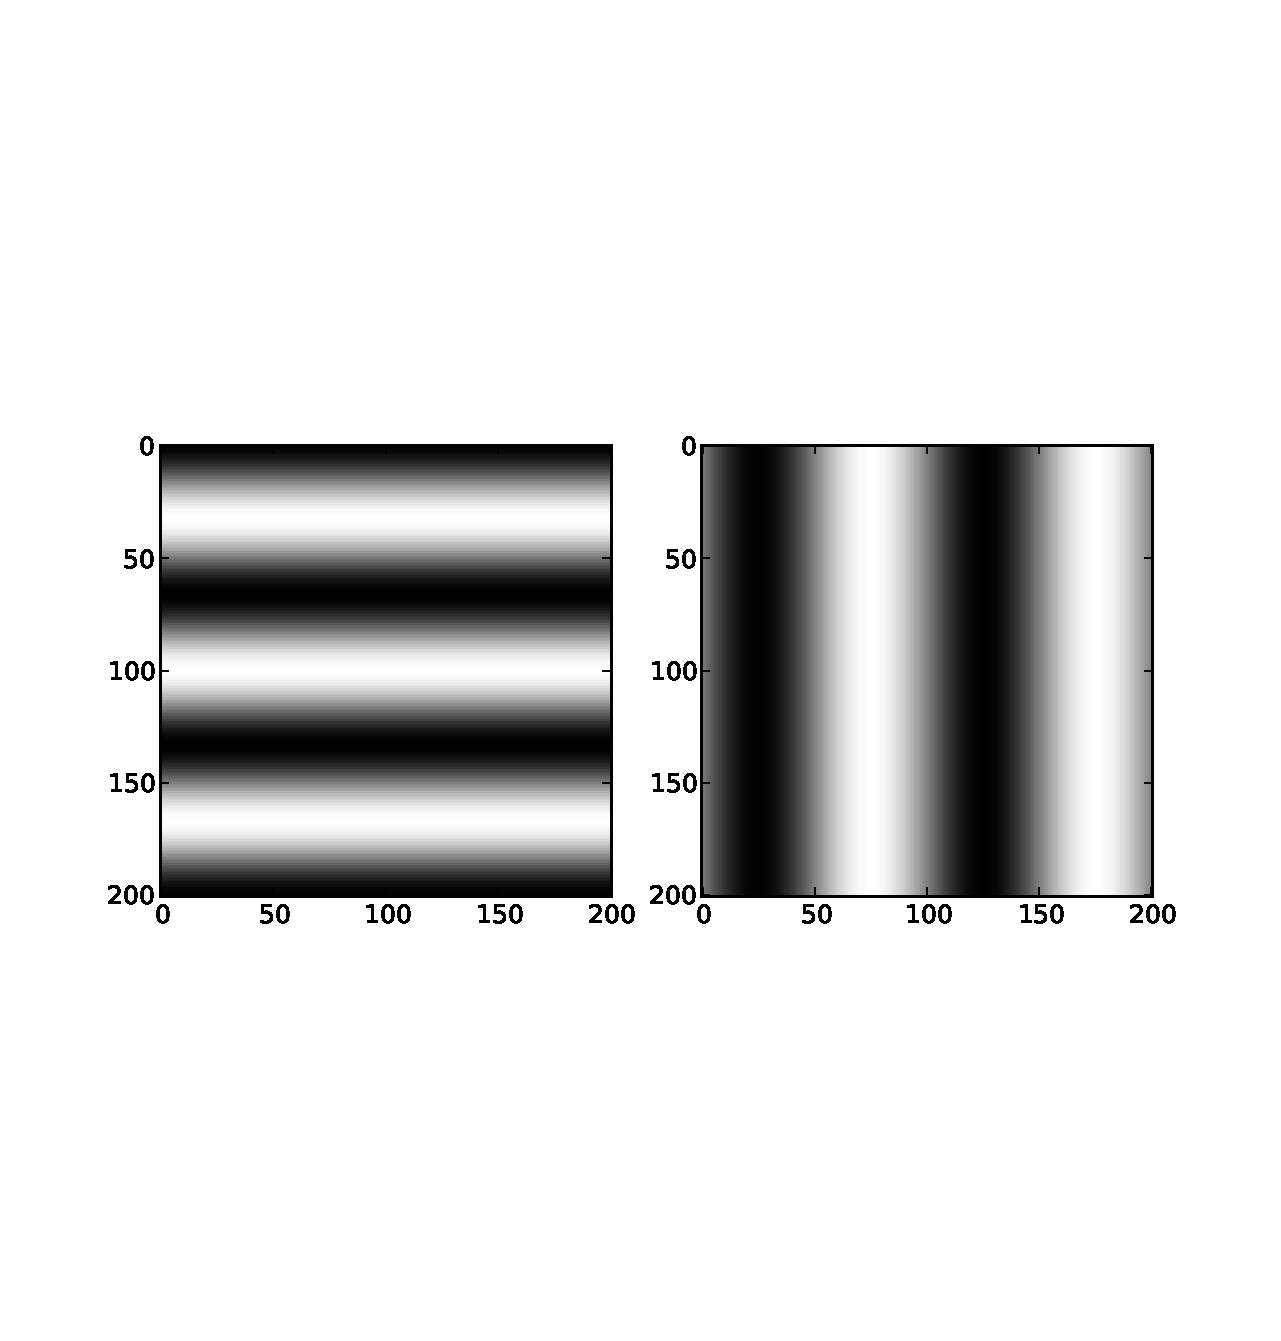
\includegraphics[width=0.5\textwidth]{../images/0_fx_and_fy}
          \caption{Fx and Fy}
        \end{figure}

    \subsection{Plot gradient vectors}

        \begin{figure}
          \centering
          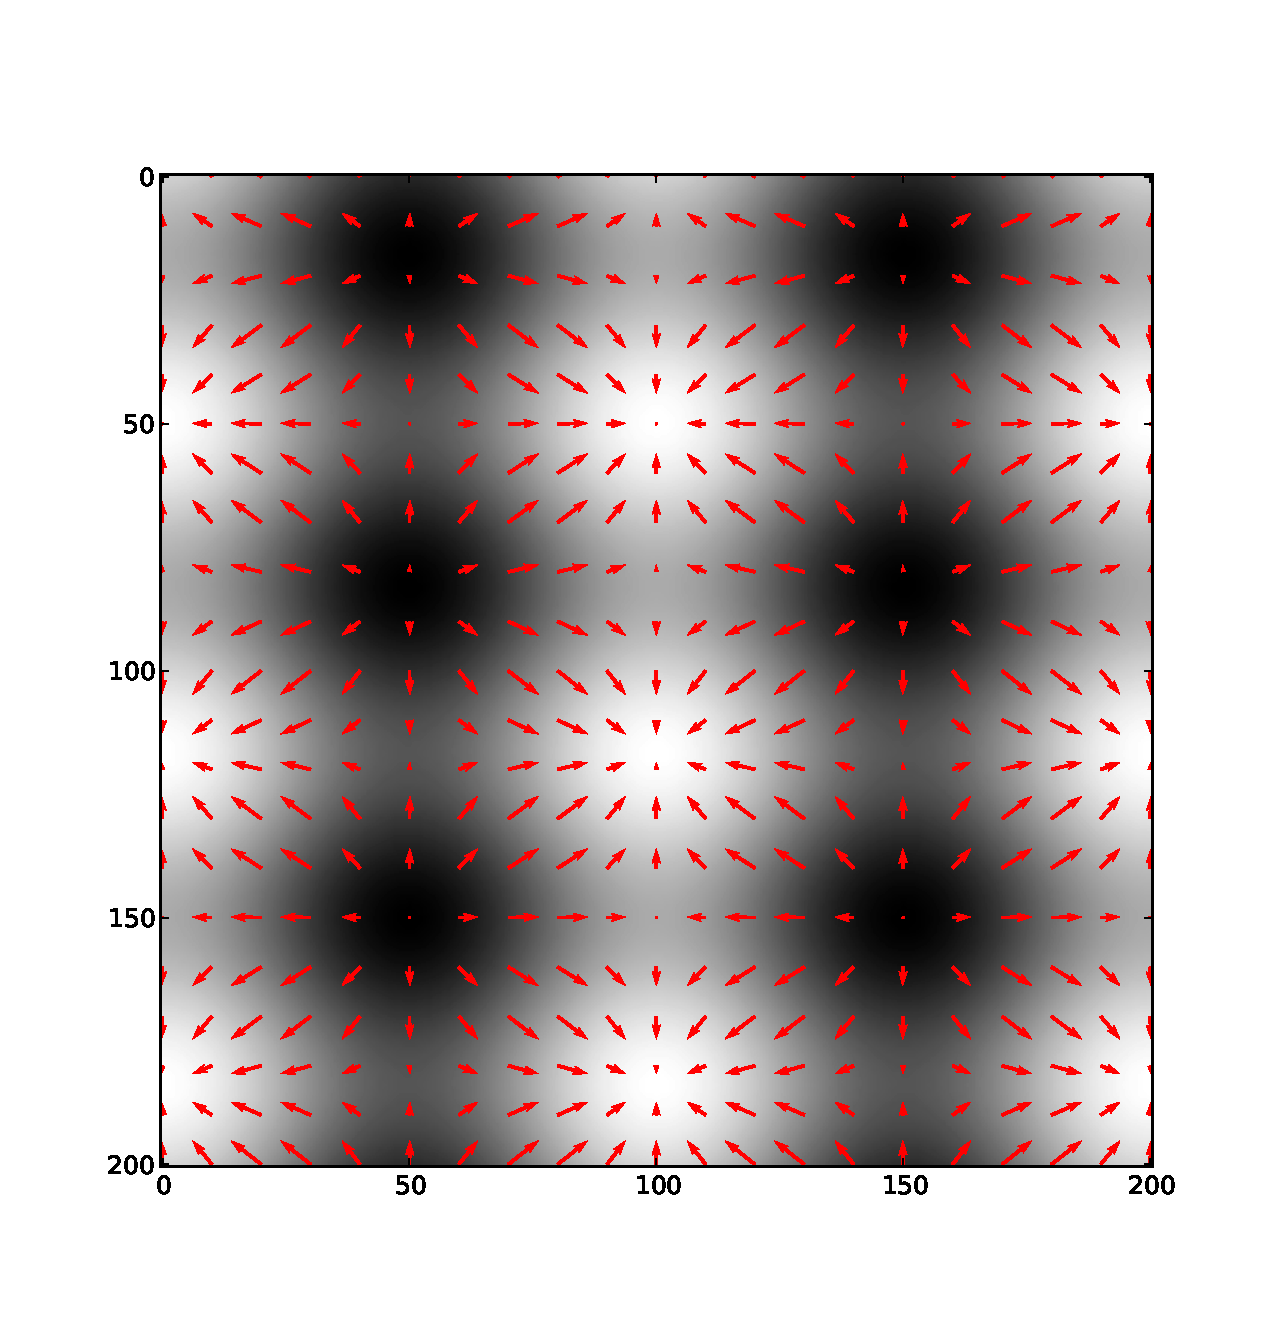
\includegraphics[width=0.5\textwidth]{../images/1_quiver}
          \caption{Gradient vectors for F}
        \end{figure}


\section{Gaussian convolution}

    \subsection{Implement \texttt{gauss(s)} function}

        \subsubsection{Code}

            \begin{verbatim}
        
    def gauss(s):
        """ Gaussian kernel with scale s and dimensions s*6+1 by s*6+1  """

        size = s * 3
        x, y = np.meshgrid(np.arange(-size,size + 1), np.arange(-size,size + 1))
        kernel = np.exp(-(x**2 / float(s) + y**2 / float(s)))
        kernel = kernel / kernel.sum()
        return x, y, kernel

            \end{verbatim}

    \subsection{Plot of kernel}

        \begin{figure}
          \centering
          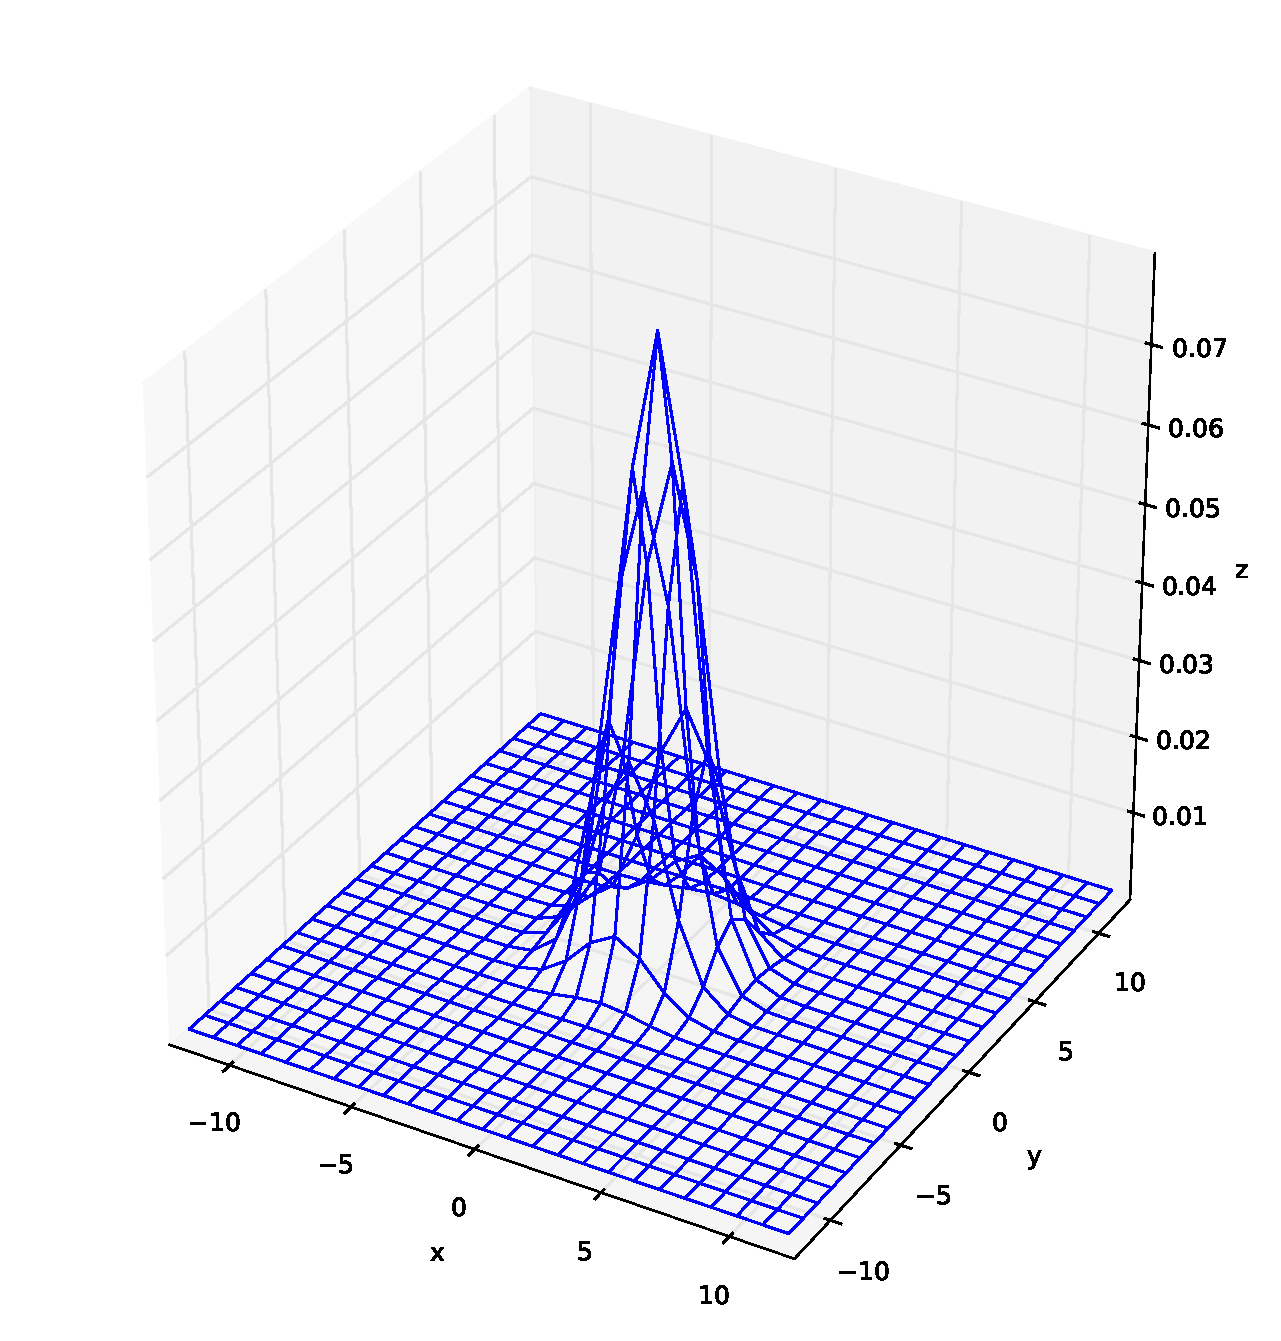
\includegraphics[width=0.5\textwidth]{../images/2_kernel3d}
          \caption{Discretised 2D Gaussian kernel}
        \end{figure}

    \subsection{Implement and time the Gaussian convolution}

        \subsubsection{code}

            \begin{verbatim}




            \end{verbatim}

        \subsubsection{Function performance plot}

            The plot in \ref{timing1} shows that the \texttt{gauss()}
            implementation is in an exponential order of complexity. 

            Note that the labels of the y-axis in the following histogram are of
            the form \texttt{convolve(cameraman, gauss([nr])[2])} where
            \texttt{gauss([nr])[2]} represents the Gaussian kernel for scale =
            [nr].
        
            \begin{figure}
              \centering
              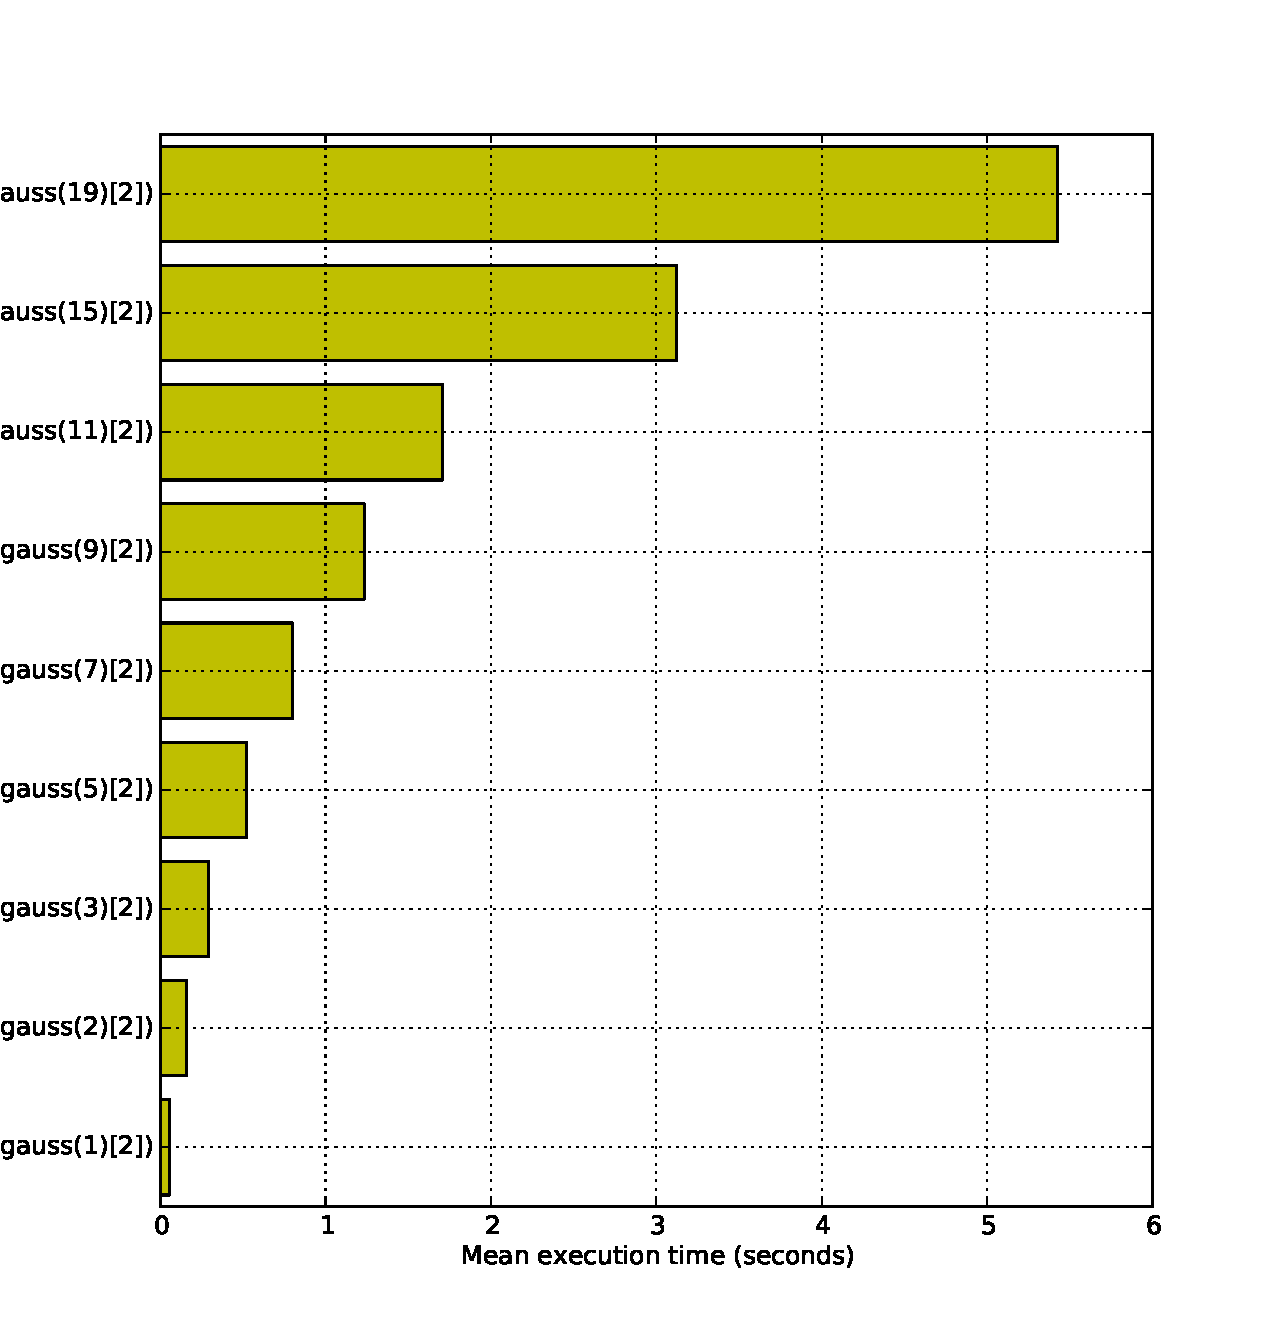
\includegraphics[width=0.5\textwidth]{../images/3_time_gauss}
              \caption{Timing of gauss() based convolution against s}
              \label{timing1}
            \end{figure}


\section{Separable Gaussian convolution}

    \subsection{Implement \texttt{gauss1()} function}

    \subsection{Obtain Gaussian convolution}


\section{Gaussian derivatives}

    \subsection{Show that derivatives of 2d Gauss function are separable}
    
    The general 1d Gaussian functions has the form 
    $ f(x) = a e^{- { \frac{(x-b)^2 }{ 2 c^2} } } $ 
    and the general 2d function has the form 
    $ f(x,y) = a e^{- \left(\frac{(x-x_o)^2}{2\sigma_x^2} + \frac{(y-y_o)^2}{2\sigma_y^2} \right)} $. 
    We use the 1d Guassian function with a = 1, b = 0, and $ 2\sigma_x^2 = s $ and
    we use the 2d Gaussian funtion with a = 1, $ x_0 = y_0 = 0 $ and $ 2\sigma_x^2 = s $.\\
    \\
    In the Separable Gaussian convolution section we have shown that we can express the
    2d convolution as a multiplication of the two 1d convolutions. With this 
    basis, we can show that the all derivatives are of the the 
    same form, but with different constants since we are deriving an exponential
    function. This is import because the derivative of $e^x$ is $e^x$. This 
    means that the function continues to be a Gaussian function no matter how
    many times and no matter over witch dimension we derive. \\
    \\
    To show this we derive our Gaussian function analytically in both dimensions 
    up to the second order.\\
    \begin{align*}
    &f(x,y)   =  e^{ (-\frac{(x)^2 +(y)^2}{s})} \\
    &f(x,y)_x =  \frac{2x}{s} e^{ (-\frac{(x)^2 +(y)^2}{s})} \\
    &f(x,y)_y = \frac{2y}{s} e^{ ( -\frac{(x)^2 +(y)^2}{s})} \\
    &f(x,y)_{xx} =  \frac{4x^2-2s}{s^2} e^{ (-\frac{(x)^2 +(y)^2}{s})} \\
    &f(x,y)_{yy} =  \frac{4y^2-2s}{s^2} e^{ (-\frac{(x)^2 +(y)^2}{s})} \\
    &f(x,y)_{xy} =  \frac{4xy}{s^2} e^{ (-\frac{(x)^2 +(y)^2}{s})}
    \end{align*}
    
    

    \subsection{Implement \texttt{gD(F, s, iorder, jorder)} function}

    \subsection{Visualise 2-jet of cameraman image}

        %\begin{figure}
        %  \centering
        %  \subfloat[air1]{\includegraphics[width=0.3\textwidth]{../images/}}                
        %  \caption{blah}
        %\end{figure}


\section{Canny edge detector}

    \subsection{Implement Canny edge detector}

    \subsection{Test Canny function on cameraman image}

        %\begin{figure}
        %  \centering
        %  \subfloat[air1]{\includegraphics[width=0.3\textwidth]{../images/}}                
        %  \caption{blah}
        %\end{figure}

        %\begin{table}
        %    \begin{tabular}{l l | *{10}{c}}
        %
        %              &Model&air2&bre1&air4&leds&air3&fire&star&air1&lbug&bre2\\  
        %        Image &     &    &    &    &    &    &    &    &    &    &    \\ 
        %        \hline
        %        lbug  &     &0.06&0.10&0.02&0.09&0.06&0.07&0.09&0.03&1.00&0.13\\  
        %        bre2  &     &0.27&0.28&0.09&0.15&0.22&0.19&0.16&0.04&0.11&1.00
        %
        %    \end{tabular}
        %    \caption{RGB intersections within database}
        %\end{table}

\end{document}
